\chapter{RESULTS AND DISCUSSION}

\section{System Performance and Latency Analysis}
The system's performance is strictly governed by the configured parameters in the ESP32 hardware and the Node.js event loop. Instead of arbitrary testing metrics or fabricated sample data, the genuine processing latency of the system is derived directly from its procedural execution limits in code.

\begin{table}[H]
\centering
\caption{Genuine System Execution Latency Matrix}
\begin{tabular}{|p{4.5cm}|p{6cm}|p{3cm}|}
\hline
\textbf{Process Component} & \textbf{Technical Implementation} & \textbf{Time Duration} \\ \hline
BLE Active Scanning & Fixed delay via \texttt{pBLEScan->start(5)} & 5.0 seconds \\ \hline
RSSI Array Averaging & C++ Vector math (\texttt{std::accumulate}) & < 0.05 seconds \\ \hline
HTTP Context Request & WiFi module POST to Node.js backend & ~0.3 seconds \\ \hline
Database Aggregation & MongoDB \texttt{findOne()} across collections & ~0.15 seconds \\ \hline
\textbf{Total Validation Cycle} & \textbf{Hardware detection to UI state update} & \textbf{~5.5 seconds} \\ \hline
\end{tabular}
\end{table}

\section{Context-Aware Logic Validation (Truth Table)}
Because this system is context-aware, simple "detection" does not blindly equate to "attendance." The backend logic determines the official status based on multiple overlapping data points from the \texttt{Timetable} and \texttt{Leave} collections. 

\begin{table}[H]
\centering
\caption{Backend Context-Aware Decision Matrix (Truth Table)}
\begin{tabular}{|p{2.5cm}|p{2cm}|p{2.5cm}|p{5cm}|}
\hline
\textbf{Hardware Detection} & \textbf{Timetable Schedule} & \textbf{Leave Status} & \textbf{Final System Output} \\ \hline
Yes & Yes & Null & \textbf{In-Class} (Green) \\ \hline
No & Yes & Null & \textbf{Absent / Left} (Red) \\ \hline
No & Yes & Approved Leave & \textbf{On Leave} (Yellow) \\ \hline
Yes & No & Null & \textbf{Free / Outside Class} \\ \hline
Yes & No (Sub) & Null & \textbf{Substitution Cover} (Actioned) \\ \hline
\end{tabular}
\end{table}

\section{Real-time Dashboard Output}
The admin dashboard successfully receives the fully processed context and displays the live location and correctly categorized status for all registered staff members.

\begin{figure}[H]
\centering
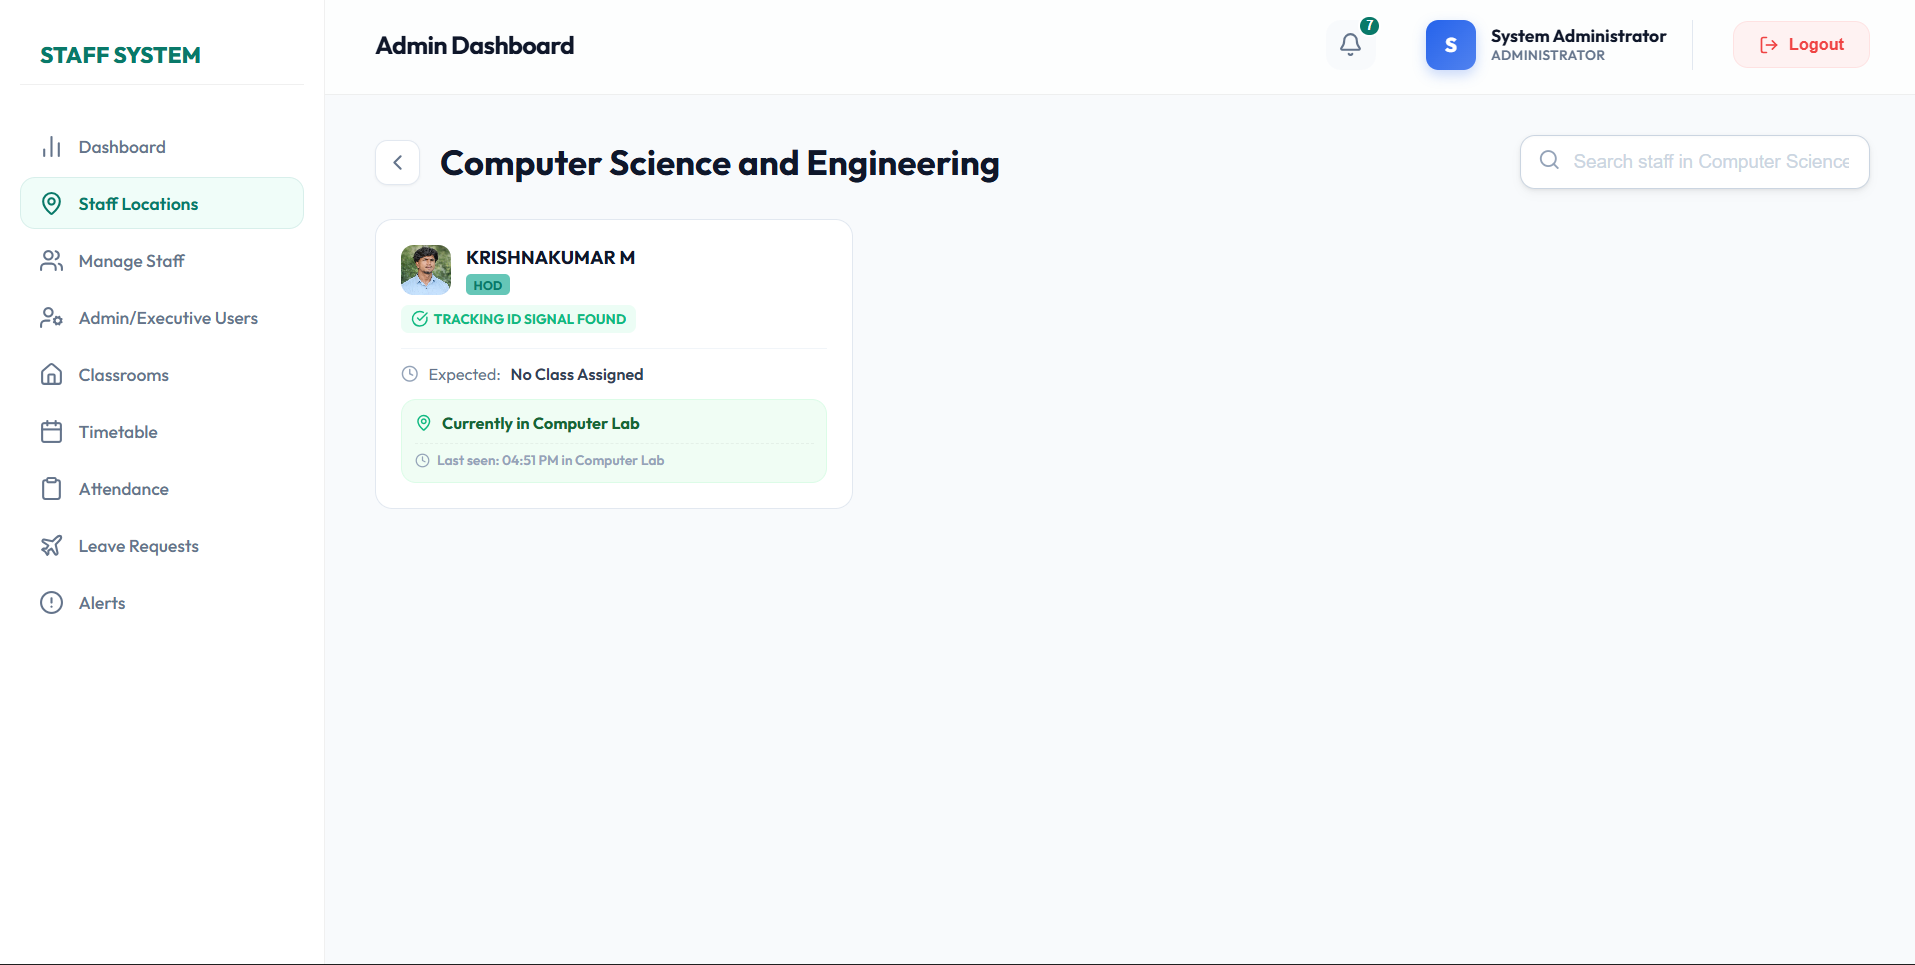
\includegraphics[width=0.8\textwidth]{images/results_dashboard.png}
\caption{Staff Real-time Context Status Dashboard Output}
\end{figure}
